\section*{Zadanie 4.}
\begin{task}
Rozważamy rozkład pola rodzaju $H_{11}$ w falowodzie prostokątnym o szerokości $a$(w kierunku osi $Ox$), wysokości $h$(w kierunku osi $Oy$). Narysować rozkłady prądów powierzchniowych oraz zaznaczyć miejsca maksimów ładunków powierzchniowych na:
\begin{enumerate}[a)]
\item ściance dolnej (y=0) oraz bocznej (x=0) przy założeniu fali bieżącej rozchodzącej się w kierunku $+Oz$
\item ściance dolnej (y=0), bocznej(x=0) oraz ściance z idealnego przewodnika przegradzającej falowód w płaszczyźnie $x=0$, przy założeniu padania fali od strony ujemnych wartości współrzędnej $z$.\\
\end{enumerate}
\end{task}

\begin{solution}

\begin{enumerate}[a)]
	\item Rozkład pól dla fali bieżącej 
	\begin{center}
	$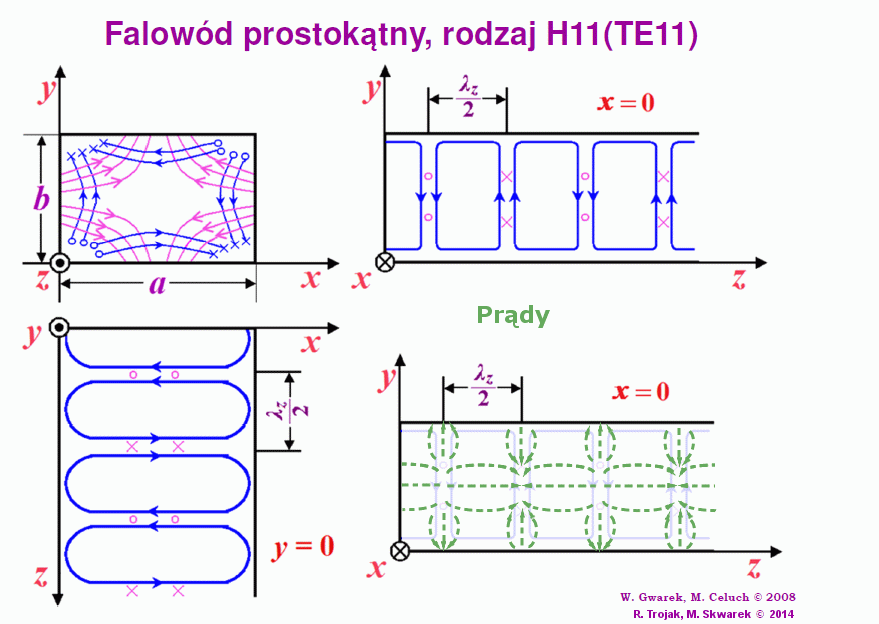
\includegraphics[scale=0.8]{4_1}$
	\end{center}


\item Rozkład pól dla fali stojącej 
	\begin{center}
	$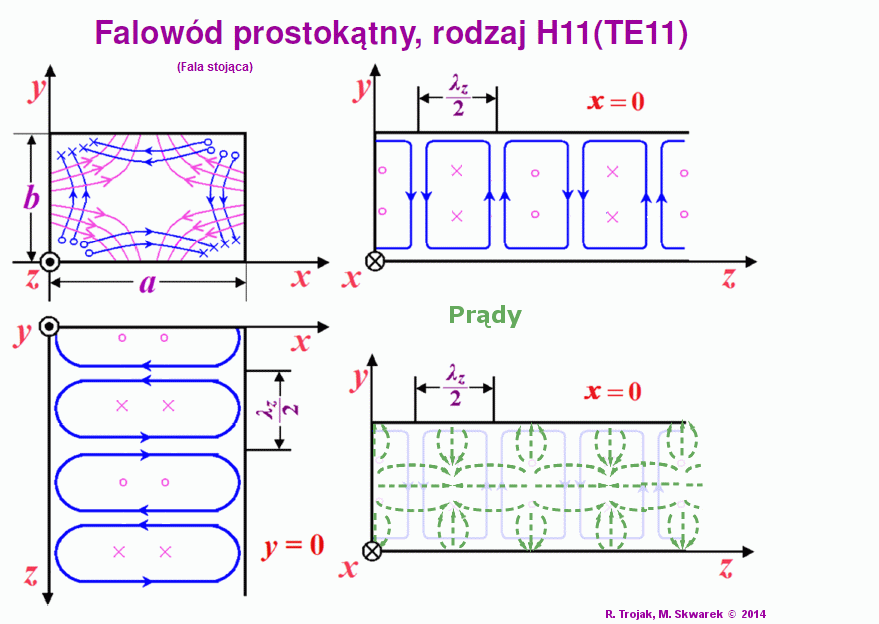
\includegraphics[scale=0.8]{4_2}$

	\end{center}

\end{enumerate}
\end{solution}